\documentclass[review]{elsarticle}

\usepackage{lineno, hyperref}
% \usepackage[hyperfootnotes=false]{hyperref}
\usepackage{array, pbox}
\usepackage{mathtools}
\usepackage{caption}
\usepackage{graphicx}
\usepackage{subcaption}
\usepackage{CJKutf8}
\usepackage[page, title]{appendix}
% \usepackage{tablefootnote}
\usepackage{threeparttable}
\usepackage{etoolbox}
\appto\TPTnoteSettings{\footnotesize}
\usepackage[bottom]{footmisc}
\usepackage{siunitx}
\usepackage{ntheorem}
\theoremseparator{:}
\newtheorem{hyp}{Hypothesis}

\usepackage{multirow}
\usepackage[normalem]{ulem}
\useunder{\uline}{\ul}{}

%to have numbered 4th level sections 1.1.1.1
\setcounter{tocdepth}{4}
\setcounter{secnumdepth}{4}

% to remove period in 4th level sections 1.1.1.1
\makeatletter
\def\els@aparagraph[#1]#2{\elsparagraph[#1]{#2}}
\def\els@bparagraph#1{\elsparagraph*{#1}}
\makeatother
% to enter a newline after 4th level sections
\newcommand{\myparagraph}[1]{\paragraph{#1}\mbox{}\smallskip}


\modulolinenumbers[5]

\journal{Tourism Management}

%% APA style
\bibliographystyle{model5-names}\biboptions{authoryear}

\begin{document}

\begin{frontmatter}

\title{Analyzing preferences differences between Chinese and English speakers in Japan hotel staying: A text mining method}

%% or include affiliations in footnotes:
\author[gidai]{Elisa Claire Alemán Carreón
\corref{mycorrespondingauthor}}
\ead{s153400@stn.nagaokaut.ac.jp}
% \orcid{0000-0002-6437-0866}

\author[gidai]{Hirofumi Nonaka}
\ead{nonaka@kjs.nagaokaut.ac.jp}

\author[gidai]{Hugo Alberto Mendoza Espa\~na}
\ead{s173330@stn.nagaokaut.ac.jp}

\author[nagasaki]{Toru Hiraoka}
\ead{hiraoka@sun.ac.jp}

\address[gidai]{Nagaoka University of Technology, Nagaoka, Japan}
\address[nagasaki]{University of Nagasaki, Nagasaki, Japan}

\cortext[mycorrespondingauthor]{
Corresponding author%: \\
% Elisa Claire Alemán Carreón \\
% Mailing Address: P.C. 940-2033, Ribbon Nagaoka B104, 1128-3 Kaminozoki-machi, Nagaoka, Niigata, Japan \\
% Cell Phone: 080-9869-4756 \\
}

\begin{abstract}
Abstract











\medskip
\noindent\it{Highlights}
\begin{itemize}
    \item Chinese customers tend to prefer included breakfasts, and rooms that are big and clean.
    \item Across all hotel prices, unsatisfied Chinese customers focus on the pricing of the hotel.
    \item English speaking customers are satisfied with the staff, cleanliness, and transportation availability.
    \item English speaking customers dislike pricey hotels and have a high dislike for dirty rooms and cigarette smell.
\end{itemize}

\end{abstract}

\begin{keyword}
Sentiment Analysis\sep Hotels and Lodging\sep Machine Learning\sep Chinese\sep English\sep Preferences
\end{keyword}

\end{frontmatter}

\linenumbers

\section{Introduction}\label{intro}

Recently, the Japanese economy has been more and more affected by an increase in inbound international tourism \cite[][]{jones2009} with a Year-on-Year Growth Rate of 19.3\% in 2017, with a total of \num[group-separator={,}]{28691073} inbound tourists that year \cite[][]{jnto2003-2019}. From this total, the tourist population was mostly Asian (86.14\%), with approximately a fourth of the total (25.63\%) coming from China. Western countries, counting English speaking countries in addition to the whole of Europe make for 11.4\% of the total, with a 7.23\% of the total being countries where English is the official or the de facto national language. Specifically for Chinese tourists, the effect on international economies as well as the number of researchers interested in this phenomenon has been increasing as well \cite[][]{sun2017}. 

However, up until recently studies on social sciences, and that includes tourist behavior, have been performed using surveys on populations that could be culturally biased for the western world \cite[][]{nielsen2017, jones2010WEIRD, guaratne2009, hogan1978biases}. Those that do include Asian populations in their analysis, most commonly Chinese tourist behavior \cite[e.g.][]{liu2019, chang2010, dongyang2015}, and a few that compare Asian to western tourist behavior \cite[e.g.][]{choi2000}, are commonly survey or interview based studies with small samples, which while valid can have its limitations. 

With the advent of Web 2.0 and customer review websites, researchers realized the benefits of online reviews for research, and their importance for sales  \cite[][]{ye2009, basuroy2003}, customer consideration \cite[][]{vermeulen2009} and perception of services and products \cite[][]{browning2013}, among other effects of online interactions between customers \cite[e.g.][]{xiang2010, ren2019}. Consequentially, tourism research also began to use information collected online for data mining analysis, such as opinion mining \cite[e.g.][]{hu2017436}, predicting hotel demand from online traffic \cite[][]{yang2014}, recommender systems \cite[e.g.][]{loh2003}, and more. Data mining and big data methodologies can increase the number of samples from the hundred or so samples manageable by researchers to the hundreds of thousands that are automatically analyzed by machines. This can not only help confirm existing theories, but also lead to finding new patterns and to knowledge discovery \cite[][]{fayyad1996data}. 

In this study we take advantage of the availability of enormous amounts of data online for Chinese and western English speaking tourist populations' online reviews for Japanese hotels to both confirm existing theories about their differences in behavior, as well as perform an exploration of the data to discover factors that could have been missed in the past. For this purpose, we use machine learning to automatically classify review sentences as positive or negative opinions of the hotel, and perform a statistical extraction of the topics that the customers of each population are most concerned about.


\section{Research objective}\label{research_objective}

The objective of this study is to determine the difference in preferences between Chinese speaking customers and English speaking customers of Japanese Hotels using text-mining techniques. In the past, survey based studies have provided a theoretical background for specific customer groups, and cultural and language differences often cannot be observed in a single study. We propose to use large scale data from online hotel reviews in Chinese and English to study these differences in a statistical manner.

These difference in preferences can become the focal point for making improvements in tourism and service industries, increase the satisfaction of customers, and influence newer customers to write more satisfied online reviews that will in turn increase sales and attract new customers.

\section{Theoretical background and hypothesis development}\label{theory_hypothesis}

\subsection{Customer satisfaction and dissatisfaction during hotel lodging}\label{theory_satisfaction}

Customer satisfaction in tourism has been analyzed since decades past, \cite{hunt1975} having defining customer satisfaction as the realization or overcoming of expectations towards the service. \cite{oliver1981} defined it as an emotional response to the provided services in retail and other contexts, and \cite{oh1996} reviewed the psychological processes of customer satisfaction for the hospitality industry. It is generally agreed upon that satisfaction and dissatisfaction stem from the individual expectations of the customer, and as such, \cite{engel1990} states that satisfaction and dissatisfaction are therefore influenced by each customer's background. This is why Western and Asian, specifically Chinese, customers can have very different factors of satisfaction and dissatisfaction since they have different backgrounds and cultures. These different backgrounds will lead to different expectations of the services that a hotel can provide for them, the experiences they should have while staying at a hotel, and the level of comfort that they will have, from the moment that they choose the hotel throughout their stay. These differing expectations in turn, will determine the differing factors of satisfaction and dissatisfaction for each kind of customer, as well as the order in which they prioritize them.
Therefore we propose our first and second hypothesis:

\begin{hyp}
\label{hyp:1}
Chinese and Western tourists have different satisfaction and dissatisfaction factors.
\end{hyp}

\begin{hyp}
\label{hyp:2}
Chinese and Western tourists have different priorities when it comes to similar satisfaction and dissatisfaction factors.
\end{hyp}

Studies on customer satisfaction \cite[e.g.][]{truong2009, romao2014, wu2009} commonly use the Likert scale \cite[][]{likert1932technique} (e.g. 1 to 5 scale from strongly dissatisfied to strongly satisfied) to perform statistical analysis of which factors relate most to satisfaction on the same dimension as dissatisfaction \cite[e.g.][]{chan201518, choi2000}. This leads to correlation analyses (either multivariate or single variable ones) where one factor can lead to satisfaction, while it is implied that the lack of it can lead to dissatisfaction. However, a binary distinction (satisfied or dissatisfied) could allow us to analyze the factors that solely correlate to satisfaction, as well as exploring factors which are solely linked to dissatisfaction. There are fewer examples of this approach, but studies have also done this in the past \cite[e.g.][]{zhou2014}. While it is true that this method can decrease the extent to which we can analyze degrees of satisfaction or dissatisfaction, it has the benefit that it can be applied to a large sample of text data via sentiment classification techniques. 

Previous research has also focused on factors that are controllable by the hotel managers and staff, i.e. hotel services, staff behavior, or facilities \cite[e.g.][]{shanka2004, choi2001}, while the satisfaction might also be influenced by factors that are uncontrollable by the hotel staff, such as surroundings, location, language immersion of the country as a whole, or of touristic destinations, as well as integration of the hotel with tours available nearby, among other factors that can play a part in the customers choice behavior and satisfaction. 
This leads to our third hypothesis:

\begin{hyp}
\label{hyp:3}
Satisfaction and dissatisfaction stems from both internal (managerial) and external (environmental) attributes of the hotel.
\end{hyp}

\subsection{Chinese and Western tourist behavior}\label{theory_zh_en}

% Asians vs Western behavior
In the past, tourist behavior analyzed from western samples and surveys was wrongly thought to be a representation of universal behavior across all cultures \cite[][]{nielsen2017, jones2010WEIRD, guaratne2009, hogan1978biases}. Recently, however, with the rise of Chinese outbound tourism, both academic researchers and businesses have decided to study Chinese tourist behavior \cite[][]{sun2017}. This results in a number of studies focusing on only the behavior of this subset of tourists. To this day, cross-cultural studies and analyses for Asian and Western tourists have been scarce. A few examples are \cite{choi2000}, where it was found that Western tourists visiting Hong Kong are satisfied more with room quality while Asians are satisfied with value for money; \cite{bauer1993changing}, where Westerners prefer the hotel health facilities while the Asian tourists were more inclined to peruse the Karaoke facilities of hotels, and both groups tend to have high expectations about facilities; \cite{kim2000}, where American tourists were found to be individualistic and motivated by novelty, while Japanese tourists were found to be collectivist and motivated by prestige and family, with escape from routine and an increase in knowledge as a common motivator. One thing to note with the above cross-culture analyses is that they were performed before around the year 2000. The current Chinese economy boom should make an increase in influx, but the question that could be made is if that boom created a difference in the expectations of tourists and as such, of their satisfactions and dissatisfactions when traveling.

% Universal behavior
Other more recent studies, perhaps recognizing that samples being comprised of people from Western industrialized countries isn't representative, have gone further and studied people from many countries in their samples, and performing a more universal and holistic (not cross-culture) analysis. \cite{choi2001}, for example, analyzed hotel guest satisfaction determinants in Hong Kong with surveys in English, Chinese and Japanese translations, with people from many countries in their sample. \cite{choi2001} found that staff service quality, room quality and value for money were the top satisfaction determinants. For another example, \cite{Uzama2012} produced a typology for foreigners coming to Japan for tourism, without making distinctions for their culture, but their motivation in traveling in Japan. In another study, \cite{zhou2014} analyzed hotel satisfaction using English and Mandarin online reviews from guests staying in Hangzhou, China coming from a number of different countries; although the factors were analyzed in general without much cross-cultural analysis, although their general satisfaction score was noticed to be different. \cite{zhou2014} thus found that customers are universally satisfied by welcome extras, dining environments and special food services. 

% Western behavior 
Regarding Western tourist behavior, a few examples can tell us what to expect when analyzing our data. \cite{kozak2002} found that British and German tourists' satisfaction determinants while visiting Spain and Turkey were hygiene and cleanliness, hospitality, the availability of facilities and activities, and accommodation services. \cite{shanka2004} found that English speaking tourists in Perth, Australia were most satisfied with staff friendliness, efficiency of check-in and check-out, restaurant and bar facilities and lobby ambiance. 

% Chinese behavior
Regarding outbound Chinese tourists, academic studies about Chinese tourists have increased \cite[][]{sun2017}. In general Chinese tourist populations have been found to have specific attributes by different researchers. According to \cite{ryan2001} and their study of Chinese tourists in New Zealand, Chinese tourists prefer nature, cleanliness and scenery in contrast to experiences and activities. With some overlap, \cite{dongyang2015} studied Chinese tourists in the Kansai region of Japan, and found that Chinese tourists are satisfied mostly with exploring the food culture of their destination, cleanliness and staff. Studying Chinese tourists in Vietnam, \cite{truong2009} found that Chinese tourists are highly concerned with value for money. According to \cite{liu2019}, Chinese tourists tend to have harsher criticism when compared with other international tourists. And according to \cite{gao2017chinese} who analyzed Chinese tourists and their connection to nature while traveling in different generations, Chinese tourists prefer nature overall, but the younger generations seems to do so less than their older counterparts. 

% Studies are not universal.
Although the studies focusing on only Chinese tourists or only Western tourists have a narrow view, their theoretical contributions are valuable. We can see that depending on the study and the design of questionnaires, the as well as the destinations, the results can vary greatly. Not only that but while there seems to be both some overlap in most studies, some factors are completely ignored in one study while not in the other.  However, with data mining, the definition of each subject or factor is left for the review writers to decide en masse, and be selected through statistical methods alone. This can open opportunities to find factors that the writers of this study would not have contemplated, or avoid enforcing a factor on the mind of reviewers by presenting them with a question that they didn't think of by themselves. In addition, this study could help us compare the satisfaction and dissatisfaction factors cross-culturally and compare them with the existing literature.

\subsection{Data mining, knowledge discovery and sentiment analysis}\label{theory_data}

% Explain data mining and discovery of theory inside the data
In the current world, data is presented to us in larger and larger quantities. What was commonly only seen in very specialized large laboratories with super computers a couple of decades ago is now common data size for market and managerial studies, independent university students and any scientist that can connect to the Internet. Such quantities of data are available to study now more than ever, but it would be impossible for researchers to parse all of this data by themselves. As \cite{fayyad1996data} summarizes, data by itself is unusable until it goes through a process of selection, preprocessing, transformation, mining and evaluation, and only then it can be established as knowledge. With the tools available to us in the are of information science, algorithms can be used to detect patterns that would take researchers too long to recognize, which can be evaluated to generate knowledge. This process is called Knowledge Discovery in Databases. 

% Text mining 
Now, there are of course many sources of numerical data to be mined, but perhaps what is most available and interesting to managerial purposes is the resource of customers' opinions in text form. With the introduction of Web 2.0, a never before seen quantity of valuable information is being posted to the Internet at a staggering speed. Text mining then, has been proposed more than a decade ago to utilize this data \cite[e.g.][]{rajman1998text,nahm2002text}, using what is called Natural Language Processing to parse language in a way that it can be analyzed by a computer, and improved on with the years. This has been used in the field of hospitality as well for many purposes, including satisfaction analysis from reviews \cite[e.g][]{berezina2016, xu2016, xiang2015, hargreaves2015, balbi2018}, social media's influence on travelers \cite[e.g.][]{xiang2010}, review summarization \cite[e.g.][]{hu2017436}, perceived value of reviews \cite[e.g][]{FANG2016498}, and even predicting hotel demand using web traffic data \cite[e.g][]{yang2014}.

% Sentiment Analysis
More than only analyzing patterns within the text, researchers have found how to determine the sentiment behind a statement based on speech patterns, statistical patterns, and other methodologies. This is called sentiment analysis, or opinion mining, and a precursor of this method was attempted since decades before \cite[][]{stone1966general}. With sentiment analysis, one could use patterns in the text to determine whether a sentence was being said with a positive opinion, a critical opinion, or even other ranges of emotions, depending on the thoroughness of the algorithm. Examples of sentiment analysis include ranking products through online reviews \cite[e.g][]{liu2017149, zhang2011}, predicting political poll results through opinions in Twitter \cite[][]{oconnor2010}, and so on. In the hospitality field, it has been used to classify reviewers' opinions of hotels in online reviews \cite[e.g.]{kim2017362, alsmadi2018}. 

% Data exploration
Because the methodology for finding patterns in the data is automatic and statistical in nature, it is both reliable, in that the algorithm will find a pattern by its nature, and unpredictable, in that because it has no intervention from the researchers in making questionnaires it can have different results from anything that the researchers could expect. This is why, much like actual mining, data mining is mostly exploratory in nature. One can never be sure that something can be found, but we can make predictions and estimates about where to find knowledge, and what kind of knowledge can be uncovered. 

In this study, we can predict that several things might occur. Our data could show satisfaction and dissatisfaction factors that are universal and it could also find strictly cultural preferences, but we expect that both of these options will present themselves. We can also assert that, if the previous literature is correct in their findings, we could arrive to very similar results, albeit using a database several orders of magnitude larger. We can also expect that, because of the lack of questionnaire design and freedom of users to record their pleasures and grievances, it is possible that we will discover patterns that were previously unnoticed by researchers.

\section{Methodology}\label{method}

We have extracted a large number of text reviews from a Chinese portal site \textit{Ctrip}\footnote{\label{ctrip}Ctrip: \href {www.ctrip.com/}{\path{www.ctrip.com/}}}, as well as the travel site \textit{TripAdvisor}\footnote{\label{tripadvisor}TripAdvisor: \href {www.tripadvisor.com/}{\path{www.tripadvisor.com/}}} and determined the most commonly used words that would contribute the most to positive and negative opinions in a review using Shannon's entropy to extract keywords from their vocabulary. These positive and negative keywords allow us to perform a Support Vector Machine based emotional classification of the reviews in large quantities, saving time and resources for the researchers. After classifying the sentences in the extracted reviews as emotionally positive or negative with an optimized SVM, we also observed their weight values in the machine, and the frequency of the terms in all of the reviews to extract the most utilized words in either kind of reviews. We show an overview of this methodology in Figure \ref{fig:method-overview} \cite[][]{Aleman2018ICAROB}.

\begin{figure}[bp]
\centering
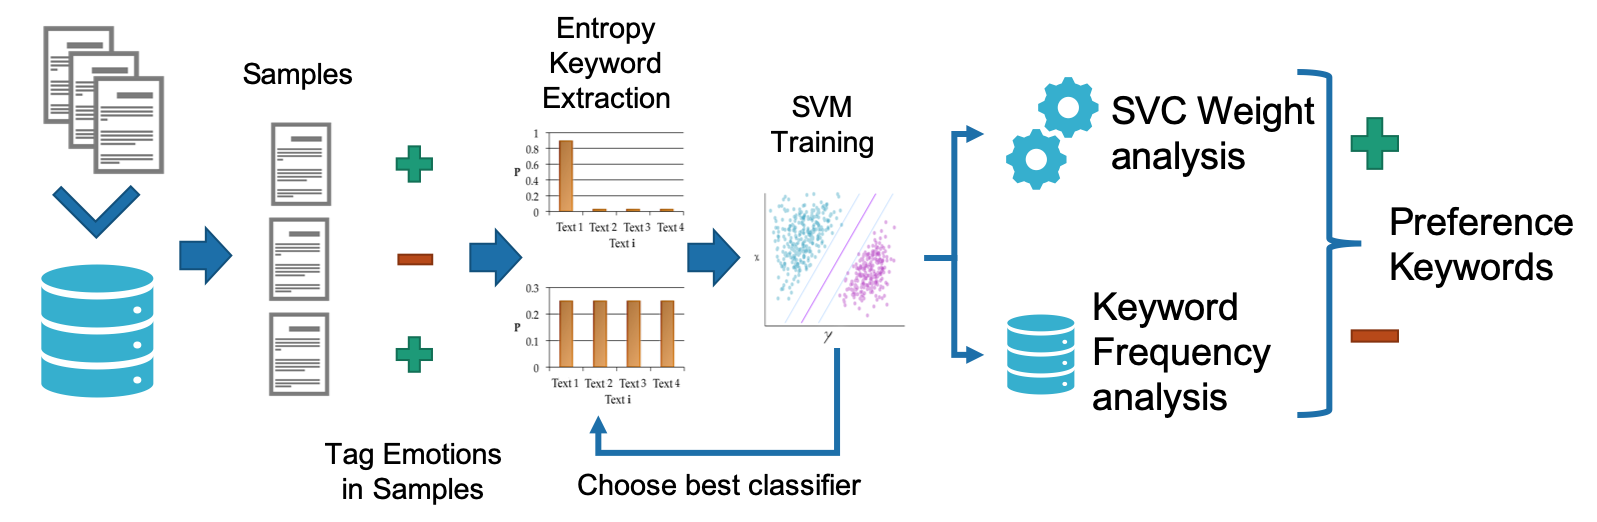
\includegraphics[width=\textwidth]{emotion-method-overview.png}
\caption{Overview of the methodology.}
\label{fig:method-overview}
\end{figure}

\subsection{Data collection}\label{datacollection}

In the data collection stage for Chinese reviews in \textit{Ctrip} a total of \num[group-separator={,}]{5938} review pages of hotels in Japan were collected. From these pages, we extracted a total of \num[group-separator={,}]{44177} reviews, which were comprised of \num[group-separator={,}]{572218} separate sentences. 

% In our corpus, there were \num[group-separator={,}]{23443} different words used, from which \num[group-separator={,}]{2802} were noise characters.

In the TripAdvisor data collection, we collected data from \num[group-separator={,}]{21154} different hotels. In total, we collected \num[group-separator={,}]{295931} reviews in English, which we then separated into \num[group-separator={,}]{2697086} sentences using the \textit{gensim} python library. 

\subsection{Text processing}\label{textprocessing}

Because Chinese text doesn't have spaces, in order to parse Chinese words on their own we used the Stanford Word Segmenter \cite[][]{chang2008} program developed by the Stanford NLP Group\footnote{\label{stanfordnlp}The Natural Language Processing Group at Stanford University}. In the case of texts in English, however, only using spaces is not enough to correctly collect concepts. Because of variations and conjugations of words depending on the context and tense, a better segmentation is achieved by using lemmatization, which returns the dictionary form of each word. For this purpose, we used the \textit{gensim} library with the English texts.

\subsection{Sentiment analysis}\label{sentimentanalysis}

The sentiment analysis was performed using the methodology described in \cite{Aleman2018ICAROB}. A group of keywords is determined by a calculation and comparison of Shannon's entropy \cite[][]{shannon1948} between two classes, and then the keywords are used in a Support Vector Classifier \cite[][]{cortes1995}, optimizing the entropy comparison values to select the best performing classifier. The selected classifier's feature keywords would then clearly represent the user preferences leading to positive and negative emotions.

Shannon’s entropy, in the field of Information Theory, is defined to be the expected value of the information content in a signal. It is shown in formulas \ref{eq:H} and \ref{eq:lim_H}. Using this value we can observe the probability distribution of each word inside the corpus. A word that is included in many documents will have a high entropy value for that set of documents. Opposite to this, a word appearing in only one document will have an entropy value of zero. We show this concept in Figure \ref{fig:entropygraphs}.

\begin{equation}\label{eq:H}
H = - \sum_{i=1}^M [P \log_2 P]
\end{equation}

\begin{equation}\label{eq:lim_H}
\lim_{P\to0+} P \log_2 P = 0
\end{equation}

\begin{figure}[bp]
    \centering
    \begin{subfigure}[b]{0.4\linewidth}
        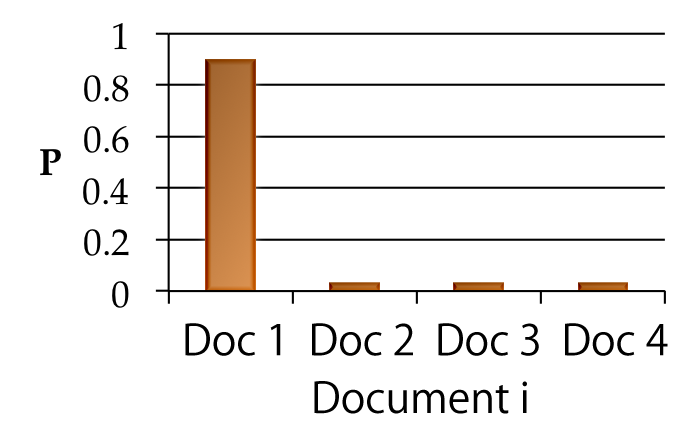
\includegraphics[width=\linewidth]{entropyzero.png}
        \caption{Entropy close to zero.}
    \end{subfigure}
    \begin{subfigure}[b]{0.4\linewidth}
        \includegraphics[width=\linewidth]{entropyhigh.png}
        \caption{High entropy}
    \end{subfigure}
\caption{Probabilities of a word j being contained in a document i.}
\label{fig:entropygraphs}
\end{figure}

To apply this logic, we retrieved 50 reviews as a sample of our corpus and with the collaboration of a group of 5 Chinese students, which were split into 159 sentences. We then tagged each sentence as the classes positive or negative depending on the emotion that the text conveyed, then calculated the entropy values for each word in relation to the set of sentences from each class. In the case of English reviews, we sampled 665 reviews and with the collaboration of English speaking students manually tagged them by sentence, resulting in \num[group-separator={,}]{2357} tagged sentences. Words with higher entropy relating to the satisfaction set than to the dissatisfaction set by a factor of \(\alpha\) were determined to be keywords tied with satisfaction in Chinese reviews of hotels. This is shown in formula \ref{eq:entropy_pos}. Likewise, words with higher entropy for the dissatisfaction set than the satisfaction set by a factor of \(\alpha'\) were determined to be keywords tied to dissatisfaction in our texts. This is shown in formula \ref{eq:entropy_neg}. Examples of positive and negative sentences in English and Chinese are shown in the Appendix, in Table \ref{tab:training_examples}.

\begin{equation}\label{eq:entropy_pos}
H_{P} > \alpha H_{N} % \rightarrow satisfaction \: keyword
\end{equation}

\begin{equation}\label{eq:entropy_neg}
H_{N} > \alpha' H_{P} % \rightarrow dissatisfaction \: keyword
\end{equation}

The mutually independent coefficients \(\alpha\) and \(\alpha'\) were tested from 1.25 to 6 in intervals of 0.25. The result was 40 lists for each language, 20 for each emotional class. We trained a different Support Vector Classifier with each of the lists, and we chose the best performing lists for each emotional class and then combined the successful lists to train our best performing classifier. This resulted in a best performing positive emotion classifier (positive/non-positive) for each language.

For the performance tests, we used a 5-fold cross-validation \cite[][]{kohavi1995} process in the Chinese reviews, and a 10-fold cross-validation process in the English reviews case, in which we calculated their F-measure \cite[][]{powers2011} means and standard deviations. The number of \(k\)-folds was decided from the sample size. Table \ref{tab:svm_f1_zh} shows the lists that had the best performance results in the case of Chinese text and Table \ref{tab:svm_f1_en} shows the best performance results in English texts in the Appendix. 

We then used these best performing classifiers in the rest of the respective data to label positive emotion sentences in a binary manner. The sentences not belonging to the positive emotion class were considered to belong in the negative emotion class. This resulted in \num[group-separator={,}]{506452} positive Chinese sentences, \num[group-separator={,}]{65766} negative Chinese sentences, \num[group-separator={,}]{1288098} positive English sentences and \num[group-separator={,}]{1408988} negative English sentences.

\subsection{SVM weight analysis}\label{svmweightsanalysis}

During the SVM learning algorithm, each point of data that is classified incorrectly causes a change in the weight vector to better classify new data correctly. These changes to the weight vector are strong for features that needed to be taken account of to classify with a minimal error, those contained in the support vectors, close to the separating hyperplane. Sequentially, the weight vector can be interpreted as a numerical representation of the effect each feature had for each class in the classification process. Below we show the formula for the weight vector (\ref{eq:svm_weight}).

\begin{equation}\label{eq:svm_weight}
w = \sum_{i=1}^N \alpha_i y_i x_i
\end{equation}

\subsection{Rank-biased Overlap}\label{rbo}

In order to compare the similarity between two ranked lists, most cases would call to action a statistical measure such as Kendall's \(\tau\). However, since the lists are not necessarily of the same length, or have necessarily the same contents, and are top-weighted (where the first rank is the most important to know, with less and less importance as the ranks continue), it is necessary to use another measure of similarity. \cite{webber2010similarity} proposed a Rank-biased Overlap measurement, which takes all of these factors into consideration. Because our Chinese keywords (their translations, at least) don't match our English keywords one to one, it is necessary to use this method. Webber's RBO produces 3 measurements: a minimum RBO, a residual RBO (from which one can know the maximum RBO), and an extrapolated RBO (where the list is assumed to continue in the same pattern of similarity towards infinity). The formula for the extrapolated RBO is shown in (\ref{eq:rbo_ext}), Where \(S\) and \(T\) are listings, \(d\) is their depth, \(k\) is their evaluation depth, \(p\) is a parameter that controls the top-weightedness of the lists (or it could be thought as \(1-p\) being the probability to stop looking at the next item in the list), and \(X\) being the overlap between the lists. The complete process is described at length by \cite{webber2010similarity}.

\begin{equation}\label{eq:rbo_ext}
RBO_{EXT}(S,T,p,k) = \frac{X_k}{k} \cdot p^k + \frac{1-p}{p} \sum_{d=1}^k{\frac{X_d}{d} \cdot p^d}
\end{equation}

\section{Data Analysis}\label{dataanalysis}

% WITHOUT PERCENTAGE
\subsection{Frequent keywords and their SVM weight values}\label{svmresults}

In order to understand the preferences of Chinese speaking tourists and English speaking tourists when lodging in Japan, we study both the frequency of the words they use in relation to the number of total reviews, and their weight in the SVM classifiers. In order to know the relevance of a keyword as a preference for each group, we observed the frequencies of each entropy based keyword in our complete data set and their SVM weight value. The frequency of the keywords in the database shows the level of priority it has for customers, and the weight value allows us to observe the sentiment it relates to by its positive or negative sign. We ranked the keywords by frequency, and use their SVM weight for analyzing the related sentiment (positive weight means positive sentiment, and negative weight signifies negative sentiment). 

We observed the top 10 words with the highest frequencies for keywords that were linked by entropy to satisfaction and dissatisfaction in emotionally positive and negative statements to study and quantitatively rank the needs of Chinese customers, as shown in the Tables \ref{tab:pos_keys_zh} and \ref{tab:neg_keys_zh} (however, the latter does not have more than 7 keywords available); and for English speaking customers, as shown in Tables \ref{tab:pos_keys_en} and \ref{tab:neg_keys_en}.

There were many more keywords than shown in most cases, however, and some showed to be high in weight but low in frequency. This could mean they were useful for classification (the emotional reaction is more extreme) but aren't as important a preference for users (there aren't many cases in that the keyword was applicable). In the appendix, Table \ref{tab:key_weights_zh} shows some keywords that have a relatively high weight value for both positive and negative extremes, and their translations in the relevant context. In Table \ref{tab:key_weights_en} we show keywords for the English classifier with high weight values as well.

% Chinese_frequencies_svm_weight_positive_translations_matched.csv

\begin{table}[hbp] \centering
\caption{Top 10 frequently used positive Chinese keywords in satisfaction sentences.}
\label{tab:pos_keys_zh}
\begin{tabular}{|c|l|c|c|c|} \hline
\textbf{Word} & \multicolumn{1}{c|}{\textbf{Translation}} & \textbf{Frequency} & \textbf{SVC Weight} \\ \hline
% 1
\begin{CJK}{UTF8}{gbsn} 大 \end{CJK} 
    & big 
        & 15470 & 0.624 \\ \hline
% 2
\begin{CJK}{UTF8}{gbsn} 干净 \end{CJK} 
    & clean 
        & 12166 & 0.638 \\ \hline
% 3
\begin{CJK}{UTF8}{gbsn} 早餐 \end{CJK} 
    & breakfast 
        & 10575 & 0.495 \\ \hline
% 4
\begin{CJK}{UTF8}{gbsn} 推荐 \end{CJK} 
    & recommendation 
        & 8752 & 0.495 \\ \hline
% 5
\begin{CJK}{UTF8}{gbsn} 环境 \end{CJK} 
    & \begin{tabular}[c]{@{}l@{}}
    environment
    \end{tabular} 
        & 8694 & 0.248 \\ \hline
% 6
\begin{CJK}{UTF8}{gbsn} 周边 \end{CJK} 
    & periphery 
        & 8456 & 0.495 \\ \hline
% 7
\begin{CJK}{UTF8}{gbsn} 近 \end{CJK} 
    & close
        & 8372 & 0.028 \\ \hline
% 8
\begin{CJK}{UTF8}{gbsn} 交通 \end{CJK} 
    & transportation
        & 8264 & 0.586 \\ \hline
% 9
\begin{CJK}{UTF8}{gbsn} 附近 \end{CJK} 
    & nearby
        & 6619 & 0.495 \\ \hline
% 10
\begin{CJK}{UTF8}{gbsn} 地铁 \end{CJK} 
    & subway
        & 5386 & 0.180 \\ \hline
\end{tabular}
\end{table}

% Chinese_frequencies_svm_weight_negative_translations_matched.csv

\begin{table}[hbp] \centering
\caption{Frequently used negative Chinese keywords in dissatisfaction sentences.}
\label{tab:neg_keys_zh}
\begin{tabular}{|c|l|c|c|} \hline
\textbf{Word} & \multicolumn{1}{c|}{\textbf{Translation}} & \textbf{Frequency} & \textbf{SVC Weight} \\ \hline
% 1
\begin{CJK}{UTF8}{gbsn} 价格 \end{CJK} 
    & price 
        & 7636 & -1.505 \\ \hline
% 2
\begin{CJK}{UTF8}{gbsn} 地理 \end{CJK} 
    & geography 
        & 2238 & -0.812 \\ \hline
% 3
\begin{CJK}{UTF8}{gbsn} 中文 \end{CJK} 
    & Chinese language 
        & 1410 & -0.714 \\ \hline
% 4
\begin{CJK}{UTF8}{gbsn} 陈旧 \end{CJK} 
    & old-fashioned 
        & 698 & -0.000 \\ \hline
% 5
\begin{CJK}{UTF8}{gbsn} 距离 \end{CJK} 
    & distance 
        & 349 & 0 \\ \hline
% 6
\begin{CJK}{UTF8}{gbsn} 老 \end{CJK} 
    & old 
        & 311 & 0 \\ \hline
% 7
\begin{CJK}{UTF8}{gbsn} 华人 \end{CJK} 
    & Chinese person 
        & 16 & -0.238 \\ \hline
\end{tabular}
\end{table}


% Hugo_1_SVM_Combined_p1.5_n4.25_c2_Frequency_counts_posinega_subject-only.csv


\begin{table}[hbp]
\centering
\caption{Top 10 positive English keywords in satisfaction sentences.}
\label{tab:pos_keys_en}
\begin{tabular}{|l|c|c|}
\hline
\multicolumn{1}{|c|}{\textbf{Word}} & \textbf{Frequency} & \textbf{SVC Weight} \\ \hline
% 1
staff & 138677 & 0.537 \\ \hline
% 2
clean & 105971 & 1.886 \\ \hline
% 3
location & 103151 & 0.842 \\ \hline
% 4
helpful & 63558 & 1.999 \\ \hline
% 5
comfortable & 62793 & 1.724 \\ \hline
% 6
friendly & 57307 & 1.199 \\ \hline
% 7
recommend & 51433 & 1.158 \\ \hline
% 8
train & 45148 & -0.000 \\ \hline
% 9
free & 42084 & 0.734 \\ \hline
% 10
subway & 38354 & 1.951 \\ \hline
\end{tabular}
\end{table}

% Hugo_1_SVM_Combined_p1.5_n4.25_c2_Frequency_counts_posinega_subject-only.csv

\begin{table}[hbp]
\centering
\caption{High negative weight English keywords in dissatisfaction sentences.}
\label{tab:neg_keys_en}
\begin{tabular}{|l|c|c|}
\hline
\multicolumn{1}{|c|}{\textbf{Word}} & \textbf{Frequency} & \textbf{SVC Weight} \\ \hline
% 1
pricey & 3809 & -1.614 \\ \hline
% 2
carpet & 3683 & -0.507 \\ \hline
% 3
slow & 3177 & -1.281 \\ \hline
% 4
dirty & 2943 & -1.275 \\ \hline
% 5
uncomfortable & 2942 & -2.423 \\ \hline
% 6
stain & 2787 & -1.886 \\ \hline
% 7
cigarette & 2468 & -0.435 \\ \hline
% 8
curtain & 2032 & -0.224 \\ \hline
% 9
paper & 2029 & -0.503 \\ \hline
% 10
renovation & 1898 & -0.548 \\ \hline
\end{tabular}
\end{table}

\subsection{Rank-biased Overlap}\label{rboresults}

In order to calculate the similarity between the ranked lists shown in Tables \ref{tab:pos_keys_zh} and \ref{tab:pos_keys_en}, and the lists in Tables \ref{tab:neg_keys_zh} and \ref{tab:neg_keys_en}, we calculated the extrapolated Rank-biased Overlap between the English keyword lists and the English translation of the Chinese keyword lists at different cutoff points. In addition, we prepared and modified the lists so that words that are similar but would not overlap otherwise would overlap in this analysis. For example, in the English keyword lists, the word is 'pricey' while in the Chinese keywords it is translated as 'price', and as such it was changed to 'pricey' to match the English keywords. The results of this are shown in Table \ref{tab:rbo}. In the case of Chinese dissatisfaction keywords, which is only comprised of 7 keywords, the list remains complete in all cutoff points bigger than 7, and then it is cut at the cutoff point of 5. Since the RBO measure can work regardless of the length of each list, this is not a problem in its calculation.

% Please add the following required packages to your document preamble:
% \usepackage{multirow}
\begin{table}[]
\centering
\caption{RBO results between Chinese and English ranked keyword lists, \(p=0.9\).}
\label{tab:rbo}
\begin{tabular}{|l|c|r|}
\hline
\multicolumn{1}{|c|}{\textbf{List cutoff}} & \textbf{Emotion} & \(RBO_{EXT}\) \\ \hline
\multirow{2}{*}{None} & Satisfaction & 0.222 \\ \cline{2-3} 
 & Dissatisfaction & 0.299 \\ \hline
\multirow{2}{*}{Top 20} & Satisfaction & 0.221 \\ \cline{2-3} 
 & Dissatisfaction & 0.293 \\ \hline
\multirow{2}{*}{Top 10} & Satisfaction & 0.209 \\ \cline{2-3} 
 & Dissatisfaction & 0.285 \\ \hline
\multirow{2}{*}{Top 5} & Satisfaction & 0.221 \\ \cline{2-3} 
 & Dissatisfaction & 0.321 \\ \hline
\end{tabular}
\end{table}

\section{Results}\label{results}

\subsection{Chinese tourists' satisfaction and dissatisfaction keywords}

Analyzing satisfaction keywords of Chinese hotel reviews from Table \ref{tab:pos_keys_zh}, we found that the most relevant subjects Chinese customers perceive positively are cleanliness and size, very possibly of the room they had stayed in. There is also the possibility that reviewers were praising, in general, the cleanliness of Japan’s environment, streets without litter, potable water and their culture of respecting spaces. Our results also indicate that closeness of the hotel to scenic places is highly preferred by Chinese customers. Lower in the list of priorities, other positive factors that come into play when Chinese tourists choose a hotel to stay is the location in relation to public transport availability (such as the subway); and as mentioned before, environments, such as gardens or parks nearby; and services nearby, like places to go shopping. 

One key component we found in Chinese customer preferences is the inclusion of breakfast within the hotel. This can be inferred from the high frequency with which this keyword was included in the sentences emotionally classified as positive. While other food-related words were extracted, most of them were general in nature, like “food” or “eating”, and in a lower ranking. In contrast, the word “breakfast”, which is referring to a specific time and very possibly its inclusion in the hotel commodities, was very frequently used in positive texts compared to other food-related words. 

Regarding dissatisfaction keywords in Table \ref{tab:neg_keys_zh}, we found that the most frequently criticized aspect of Japanese hotels was the price. Another important negative factor can be the availability or lack thereof of Chinese translations. Chinese customers can feel lost when they don't understand directions or instructions, either written or spoken; however, according to our data, most customers can be thought to have complained about written translations. Another dissatisfaction factor is the word 'old', which can be referring to the age of the building, or the general design and look of the place being old-fashioned.

We can assert that Chinese customers value the room quality over transportation availability, that they are interested in included breakfast with the hotel stay, that they are concerned with value for money and the availability of Chinese language translations to have an easier time in the accommodation.

\subsection{English speaking tourists' satisfaction and dissatisfaction keywords}

The most important satisfaction keyword in English reviews (see Table \ref{tab:pos_keys_en}) is 'staff', while lower in the list we can also observe 'helpful' and 'friendly', possibly referring to the staff as well, and since Japan is famous for it's customer service culture, this is not unexpected. Next on the list we can observe they value cleanliness, but a few more items in the list are regarding location of the hotel, and possibly the availability of nearby transportation, such as the subway or train. We can also observe that the word 'free' is present there, which after observing a few examples in the database, we concluded that it relates to the free amenities in a hotel room, such as cosmetics, soaps, coffee, tea, and so on.

The negative keywords of dissatisfied customer reviews (see Table \ref{tab:neg_keys_en}) reveal an interesting picture. While the most used keyword is also related to the price of the hotels, most of the keywords relate to the hygiene of the hotel, namely dirty carpets, stains, cigarette smell in the room or curtains, and so on. We can also observe that the word 'renovation' is written lower in the list. Some cities in Japan (e.g. Osaka) are currently going under a large number of renovations, which are also extending to the hotel facilities. Customers staying in places in renovation or near a renovation construction can be expected to wake up to construction noises, have their view obstructed by metal bars, and other unpleasant experiences. Another keyword there is 'slow', which upon inspection of example reviews, we concluded that it reflects the speed of the Internet connection in the hotel rooms.

We can assert that English speaking tourists value staff friendliness and location convenience in relation to transport, but are concerned about any kind of decline in room quality both visually and regarding the smell and air quality, being quick to judge any sort of remains of cigarette smell.

\subsection{Comparison of Chinese and English speaking tourists' preferences}

% USE Results from Rank-biased Overlap (full list) experiment results_p_0.9_cutoff_10.txt

The extrapolated Rank-biased Overlap (shown in Table \ref{tab:rbo}) ranged from 0.20 to 0.22 in satisfaction lists at different cutoff points, and from 0.28 to 0.32 in the dissatisfaction lists. This means that, while there is some similarity, the preferences are fundamentally different if we consider them as top-weighted, that is, the first elements are the most important in the lists, and therefore in their similarity measurement as well.

From observation however, we can assert that both Chinese and English speaking tourists in Japan have different priorities, but consider the location of the hotel and the availability of transport nearby, such as subway or trains, as a secondary but still important point in their satisfaction of a hotel. The Chinese customers are primarily satisfied with the room quality in spaciousness and cleanliness, while the English speaking customers are easily upset by any lack of cleanliness and smoke smell from cigarettes. English speaking tourists on the other hand value staff friendliness over room quality when considering their satisfaction. 

We also can observe some keywords that aren't considered by their counterparts. For example, Chinese tourists are very satisfied with breakfast inclusion, while English speaking customers are satisfied with free amenities. On the other hand, English speaking customers mentioned tobacco smell in many reviews, while it wasn't statistically identified as a problem at all for their Chinese counterparts. 

\section{Discussion}\label{discussion}

\subsection{}

% \subsection{Needs of the Chinese tourist market in Japan}\label{discussionneeds}

% Analyzing the results from the extracted keywords is the key to understanding Chinese and English speaking customers of Japanese hotels since they can be interpreted as rankings of their explicit needs and demands.

% Our results are compatible with \cite{ryan2001} in their study of Chinese tourist behavior in New Zealand , where Chinese travelers were found to prefer traveling and exploring unfamiliar places that have a reputation for being clean and unpolluted environments, focusing on scenic beauty, history and culture. They also found complaints about the lack of Chinese language availability in the services they consumed. \cite{LIU2019337} describe that the behavior studied in Australia reflected that Chinese tourists were more likely to appreciate touristic places for the scenery, architecture, landmarks, and popular spots, rather than appreciate cultural experiences or activities. Similar to the findings in Liu et al., our results indicate that closeness of the hotel to scenic places is highly tied to satisfaction. However, their research is on online reviews of touristic places, instead of hotels. With this difference, our results showed that breakfast inclusion and the size and cleanliness of rooms were also tied to satisfaction, aside from scenery. According to our data, other positive factors that come into play when Chinese tourists choose a hotel to stay is the location in relation to public transport availability; and as mentioned before, environments, such as gardens or parks nearby; and services nearby, like places to go shopping. \cite{gao2017chinese} argue that Chinese people are heavily influenced by religion and a culture that regards harmony and oneness with nature and humans, which in turn influences their tourism behavior. However, they also argue that there are generational differences and that the older generations that lived through the changes that changed the environment and caused pollution care more about the environment, and as such appreciate natural and scenic touristic spots more than younger generations.

% This specific keyword is previously unmentioned in studies regarding the eating behavior of Chinese tourists. While these studies on eating behavior are very scarce, both a study on the food preferences of Chinese tourists in Australia \cite[][]{chang2010} and an article on Chinese food culture \cite[][]{ma2015} state that even in foreign countries, Chinese people have a habit to eat Chinese food, probably because of a need for familiarity. However, the analysis of our data points to the fact that more than Chinese food as a specific concept, hotel reviews are written with general words that represent food. We would like to further study specific Chinese tourists food preferences, such as the contents of said breakfast and other meals in future work to observe the level of necessity of these particular needs.

% In their study of Chinese tourists in Vietnam, \cite{truong2009} also found both the tendency to be concerned with value for money. It is possible that concerns over value for money are a general cultural trait in the Chinese population. Applying this previous finding to our data, negativity about the pricing of hotels across all price brackets can mean they believe the price is too high for the service that they receive, regardless of their satisfaction or dissatisfaction with the service. Our results suggest that Chinese customers are expecting lower prices for whatever services they receive.  

% Another important negative factor can be the availability or lack thereof of Chinese translations. Chinese customers can feel lost when they don't understand directions or instructions, either written or spoken; however, according to our data, most customers can be thought to have complained about written translations. 






% \subsection{Comparison with English speaking tourists in Japan}

% Previous research states that 49 - 60\% of Chinese men (and 2.0 - 2.8\% of women) currently smoke or have smoked before, taken from a sample of \num[group-separator={,}]{170000} Chinese adults in 2013-2014, which is high compared to many English speaking countries \cite[][]{zhang2019tobacco, who2015tobacco}. 

% In previous research, it has been found that Chinese tourists are harsher in their negative touristic attraction reviews than other nationalities \cite[][]{LIU2019337}. Taking this into account, and the large difference in frequency between complaints about price and other elements, Chinese customers can be said to be dissatisfied with price in a disproportionate way. English speaking tourists' dissatisfaction factors, on the other hand, have less of a gap in frequency, and as such can be said to be more concerned about cleanliness related factors than price.



% \section{Conclusions and future work}\label{conclusions}

% In this study, with the purpose to understand emotional responses of Chinese customers of Japanese hotels and understand their needs, we extracted keywords from their reviews from the Chinese portal site \textit{Ctrip} using entropy calculations from a manually classified sample of our data; then we used these keywords in machine learning experiments. Using the keywords to train a linear kernel Support Vector Classifier, we obtained the highest performance \((F=0.95\pm0.01\) using both our positive and negative keywords for a binary emotional classifier.

% Using the weight vectors of our classifiers, as well as frequency of the words in our dataset, we found that Chinese customers have a preference for big and clean rooms, big thermal baths or bathhouses, expect good value for money regardless of price, that there is a lack of Chinese text translation and that they prefer hotels where breakfast is included. We also found that the friendliness of the staff increases in priority as the price and luxury of the hotel increases and that transportation is more important for customers looking for cheaper options compared to the more luxurious ones.

% For comparison, we also repeated the experiments on reviews written by English speaker tourists staying at Japanese hotels from \textit{TripAdvisor}. Observing the results we identified that English speaking customers hold a bigger contempt and negative reactions for dirty or stained rooms, but that the main concern is also the pricing of the hotels. We also found that they prefer friendly staff and transportation available from the airport or subway.

% Our results show the needs of a large and increasing segment of the customers. This would have otherwise presented difficulties with traditional methods because of language and culture barriers. The hotel industry can make use of these results to better the response from Chinese customers by focusing on improving topics they find important, such as cleanliness, the inclusion of breakfast, availability of Chinese translations in text format and so on. By doing this, satisfied users will write new reviews and thus influence future customers positively.

% In future work we plan to investigate further into this topic, extending our data set and researching for different trends for different regions of Japan and in different kinds of hotels, as well as between customers traveling alone or in groups, for fun or for work. Another point for the future of this study is to use word clusters with similar meanings instead of single words. As mentioned before, we would also study the food preferences of Chinese tourists, as well as the impact of the recommendation in different price brackets. Additionally, it would be interesting to study further into more specific emotions than the satisfaction and dissatisfaction classifications we performed in our study.

\section*{Acknowledgements}

During our research, apart from the group of Chinese students that collaborated with the training data and emotion tagging process, we received the commentary and discussion necessary to understand certain
cultural aspects that could influence the interpretation of the data, from empirical and anecdotal Chinese sources, as well as collaboration in understanding the meaning behind the words we extracted by our dear colleagues, whom we would like to show gratitude to, Mr. Zhou Liangyuan, Ms. Fan Min and Ms. Eerdengqiqige.

\medskip

Funding: This work was supported by the Japan Construction Information Center Foundation (JACIC).

\medskip

Declarations of interest: none

\clearpage

% \section*{References}

\bibliography{bibfile-emotion}

\clearpage

\appendixpage
\appendix

\section{Sentiment analysis training data examples}

% Please add the following required packages to your document preamble:
% \usepackage{multirow}
% \usepackage{graphicx}
% \usepackage[normalem]{ulem}
% \useunder{\uline}{\ul}{}
\begin{table}[hbp]
\centering
\caption{Examples of positive and negative sentences used for training SVM}
\label{tab:training_examples}
\resizebox{\textwidth}{!}{%
\begin{tabular}{|c|c|l|}
\hline
\textbf{Language} & \textbf{Emotion} & \textbf{Sentences} \\ \hline
\multirow{4}{*}{Chinese} & \multirow{2}{*}{Positive} & \begin{tabular}[c]{@{}l@{}}\begin{CJK}{UTF8}{gbsn} 酒店 的 服务 很 好 和 我 住 过 的 所有 日本 酒店 一样 各 种 隐形 服务 非常 厉害 \end{CJK}\\ (translated as: "The service of the hotel is very good. \\ All the services of the Japanese hotels I have stayed in are extremely good.")\end{tabular} \\ \cline{3-3} 
 &  & \begin{tabular}[c]{@{}l@{}} \begin{CJK}{UTF8}{gbsn} 有 一 个 后门 到 地铁站 非常 近 周边 也 算 方便 酒店 服务 和 卫生 都 很 好 \end{CJK} \\ (translated as: "There is a back door to the subway station very close to it. \\ The surrounding area is also convenient hotel service and health are very good")\end{tabular} \\ \cline{2-3} 
 & \multirow{2}{*}{Negative} & \begin{tabular}[c]{@{}l@{}} \begin{CJK}{UTF8}{gbsn} 酒店 旁边 很 荒凉 连个 便利 店 都 要 走 很远 \end{CJK} \\ (translated as: "The hotel is very bleak, \\ and you have to go very far to go to the nearest convenience store.")\end{tabular} \\ \cline{3-3} 
 &  & \begin{tabular}[c]{@{}l@{}} \begin{CJK}{UTF8}{gbsn} 唯一 不 足 是 价格 太高 \end{CJK} \\ (translated as: "The only negative is that the price is too high.")\end{tabular} \\ \hline
\multirow{4}{*}{English} & \multirow{2}{*}{Positive} & It was extremely clean, peaceful and the hotel Hosts made us feel super welcome \\ \cline{3-3} 
 &  & \begin{tabular}[c]{@{}l@{}}Location is very good, close to a main road with a subway station, a bakery,\\  a 7 eleven and a nice restaurant that is not too expensive but serves good food\end{tabular} \\ \cline{2-3} 
 & \multirow{2}{*}{Negative} & \begin{tabular}[c]{@{}l@{}}The only downside: our room was labeled 'non-smoking' \\ but our duvet reeked of smoke.\end{tabular} \\ \cline{3-3} 
 &  & A bit pricey though \\ \hline
\end{tabular}%
}
\end{table}


\section{Entropy keyword extraction experiment results}

As explained on section \ref{sentimentanalysis}, we performed experiments with different entropy values to extract keywords from the vocabulary. Then we chose the best performing classification machine based on those keywords as shown in the Tables \ref{tab:svm_f1_zh} and \ref{tab:svm_f1_en}. We also performed experiments to choose the best value of the parameter C used in SVC. C is a constant that affects the optimization process when minimizing the error of the separating hyperplane. Low values of C give some freedom of error, which minimizes false positives, but depending on the data it can increase false negatives. Inversely, high values of C will likely result in minimal false negatives, but a possibility of false positives. 

% Please add the following required packages to your document preamble:
% \usepackage{graphicx}
\begin{table}[hbp]
\centering
\caption{Best performing SVC 5-fold cross-validation Chinese text classifiers.}
\label{tab:svm_f1_zh}
\begin{tabular}{|l|l|l|l|l|}
\hline
\textbf{Keyword List} & \textbf{\begin{tabular}[c]{@{}l@{}}Classifier \\ emotion\end{tabular}} & \textbf{C} & \begin{tabular}[c]{@{}l@{}}\(F_1\) \\ \(\mu\)\end{tabular} & \begin{tabular}[c]{@{}l@{}}\(F_1\) \\ \(\sigma\)\end{tabular} \\ \hline
\begin{tabular}[c]{@{}l@{}}Satisfaction keywords \\ (\(\alpha=2.75\))\end{tabular} & \begin{tabular}[c]{@{}l@{}}Satisfaction \end{tabular} & 2.5 & 0.91 & 0.01 \\ \hline
\begin{tabular}[c]{@{}l@{}}Negative keywords \\ (\(\alpha'=3.75\))\end{tabular} & \begin{tabular}[c]{@{}l@{}}Dissatisfaction \end{tabular} & 0.5 & 0.67 & 0.11 \\ \hline
\begin{tabular}[c]{@{}l@{}}\textbf{Combined} \\ (\(\alpha\)=2.75, \(\alpha'\)=3.75)\end{tabular} & \textbf{\begin{tabular}[c]{@{}l@{}}Satisfaction\end{tabular}} & \textbf{0.5} & \textbf{0.95} & \textbf{0.01} \\ \hline
\end{tabular}
\end{table}

\begin{table}[hbp] \centering
\caption{Best performing SVC 10-fold cross-validation English text classifiers.}
\label{tab:svm_f1_en}
\begin{tabular}{|l|l|l|l|l|}
\hline
Keyword List & \begin{tabular}[c]{@{}l@{}}Classifier \\ emotion\end{tabular} & C & \begin{tabular}[c]{@{}l@{}}\(F_1\) \\ \(\mu\)\end{tabular} & \begin{tabular}[c]{@{}l@{}}\(F_1\) \\ \(\sigma\)\end{tabular} \\ \hline
\begin{tabular}[c]{@{}l@{}}Satisfaction keywords \\ (\(\alpha=1.5\))\end{tabular} & \begin{tabular}[c]{@{}l@{}}Satisfaction\end{tabular} & 1.75 & 0.82 & 0.02 \\ \hline
\begin{tabular}[c]{@{}l@{}}Dissatisfaction keywords \\ (\(\alpha'=4.25\))\end{tabular} & \begin{tabular}[c]{@{}l@{}}Dissatisfaction\end{tabular} & 3 & 0.80 & 0.03 \\ \hline
\begin{tabular}[c]{@{}l@{}}\textbf{Combined} \\ (\(\alpha\)=1.5, \(\alpha'\)=4.25)\end{tabular} & \textbf{\begin{tabular}[c]{@{}l@{}}Satisfaction\end{tabular}} & \textbf{2} & \textbf{0.83} & \textbf{0.02} \\ \hline
\end{tabular}
\end{table}

\section{Keywords with high SVM weights regardless of frequency}

There were many more keywords than shown in Tables \ref{tab:pos_keys_en} and \ref{tab:neg_keys_en}. Some showed to be high in weight but low in frequency. This could mean they were useful for classification but aren't as important a preference for users. Table \ref{tab:key_weights_zh} shows some keywords that have a relatively high weight value for both positive and negative extremes, and their translations in the relevant context. In Table \ref{tab:key_weights_en} we show keywords for the English classifier with high weight values as well.

\begin{table}[hbp] \centering
\caption{Chinese keywords with high SVM weight values regardless of frequency.}
\label{tab:key_weights_zh}
\begin{tabular}{|>{\centering\arraybackslash}m{3em}|m{10em}|>{\centering\arraybackslash}m{7em}|>{\centering\arraybackslash}m{5em}|} \hline
\textbf{Word} & \multicolumn{1}{c|}{\textbf{Translation}} & \textbf{Entropy List} & \textbf{SVC Weight} \\ \hline
\begin{CJK}{UTF8}{gbsn} 地方 \end{CJK} 
    & region, local 
        & Positive 
        & 1.343 \\ \hline
\begin{CJK}{UTF8}{gbsn} 干净 \end{CJK} 
    & clean 
        & Positive 
        & 0.638 \\ \hline
\begin{CJK}{UTF8}{gbsn} 大 \end{CJK} 
    & big, wide 
        & Positive 
        & 0.624 \\ \hline
\begin{CJK}{UTF8}{gbsn} 交通 \end{CJK} 
    & traffic, transportation 
        & Positive 
        & 0.586 \\ \hline
\begin{CJK}{UTF8}{gbsn} 热情 \end{CJK} 
    & cordial, kindness 
        & Positive 
        & 0.495 \\ \hline
\begin{CJK}{UTF8}{gbsn} 周边 \end{CJK} 
    & periphery 
        & Positive 
        & 0.495 \\ \hline
\begin{CJK}{UTF8}{gbsn} 景色 \end{CJK} 
    & scenery 
        & Positive 
        & 0.495 \\ \hline
\begin{CJK}{UTF8}{gbsn} 推荐 \end{CJK} 
    & recommendation 
        & Positive 
        & 0.495 \\ \hline
\begin{CJK}{UTF8}{gbsn} 日本 \end{CJK} 
    & Japan 
        & Positive 
        & 0.495 \\ \hline
\begin{CJK}{UTF8}{gbsn} 早餐 \end{CJK} 
    & breakfast 
        & Positive 
        & 0.495 \\ \hline
\begin{CJK}{UTF8}{gbsn} 附近 \end{CJK} 
    & nearby 
        & Positive 
        & 0.495 \\ \hline
\begin{CJK}{UTF8}{gbsn} 中文 \end{CJK} 
    & Chinese text 
        & Negative 
        & -0.714 \\ \hline
\begin{CJK}{UTF8}{gbsn} 地理 \end{CJK} 
    & geography 
        & Negative 
        & -0.812 \\ \hline
\begin{CJK}{UTF8}{gbsn} 价格 \end{CJK} 
    & price 
        & Negative 
        & -1.505 \\ \hline
\end{tabular}
\end{table}

\begin{table}[hbp]
\centering
\caption{English keywords with high SVM weight values regardless of frequency.}
\label{tab:key_weights_en}
\begin{tabular}{|l|c|c|}
\hline
\multicolumn{1}{|c|}{\textbf{Word}} & \multicolumn{1}{c|}{\textbf{\begin{tabular}[c]{@{}c@{}}Entropy\\ List\end{tabular}}} & \multicolumn{1}{c|}{\textbf{SVC Weight}} \\ \hline
bathhouse & Positive & 2.000 \\ \hline
museum & Positive & 2.000 \\ \hline
meeting & Positive & 1.997 \\ \hline
subway & Positive & 1.951 \\ \hline
cozy & Positive & 2.000 \\ \hline
convenience & Positive & 1.888 \\ \hline
clean & Positive & 1.886 \\ \hline
comfortable & Positive & 1.724 \\ \hline
dirty & Negative & -1.275 \\ \hline
policy & Negative & -1.463 \\ \hline
prepay & Negative & -1.517 \\ \hline
pricey & Negative & -1.614 \\ \hline
sticky & Negative & -2.000 \\ \hline
\end{tabular}
\end{table}


\end{document}
